\immediate\write18{tex tqft.dtx}
\documentclass{article}
\usepackage{tikz}
\usepackage{tqft}

\makeatletter
\pgfdeclareshape{test shape}{
  \savedanchor{\centerpoint}{
    \pgfmoveto{\pgfqpoint{0pt}{0pt}}
    \pgfgetlastxy{\my@x}{\my@y}
\pgftransformyscale{-1}\pgftransformrotate{90}\pgftransformshift{\pgfqpoint{1cm}{1cm}}
    \pgfmoveto{\pgfqpoint{0pt}{0pt}}
    \pgfgetlastxy{\my@xa}{\my@ya}
    \pgf@x=-\my@x\relax
    \pgf@y=-\my@y\relax
    \advance\pgf@x by \my@xa\relax
    \advance\pgf@y by \my@ya\relax
%    \showthe\pgf@x
%    \showthe\pgf@y
  }
  \anchor{center}{\centerpoint}
\backgroundpath{
\pgftransformyscale{-1}\pgftransformrotate{90}
  \pgf@process{\pgfqpoint{0pt}{0pt}}
  \pgfpathmoveto{\pgfqpoint{0pt}{0pt}}
  \pgfpathlineto{\pgfqpoint{1cm}{0pt}}
    \pgfpathellipse{\pgfqpoint{0pt}{0pt}}{\pgfqpoint{1cm}{0pt}}{\pgfqpoint{0pt}{2cm}}
  }
}
\makeatother

\begin{document}
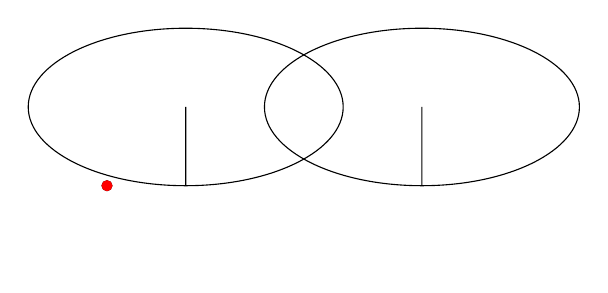
\begin{tikzpicture}
\fill (0,0) circle[radius=2pt];
\node[test shape,draw] (a) {};
\node[test shape,draw] (b) at (3,0) {};
\fill[red] (a) circle[radius=2pt];
\end{tikzpicture}

\begin{tikzpicture}[every node/.style={tqft/cobordism style={draw,thick,red}}]
 \node[
   tqft,
   fill=orange,
   fill opacity=.5,
   tqft/boundary style={fill=purple},
   tqft/cobordism style={draw,thick,red},
   tqft/boundary lower style={draw,dashed,thick,blue},
   tqft/boundary upper style={draw,green,thick},
   tqft/incoming boundary components=4,
   tqft/outgoing boundary components=6,
   tqft/offset=-1.5,
 ] (a) {};
 \fill (a incoming 2.90) circle[radius=2pt];
 \fill (a outgoing 5.270) circle[radius=2pt];
 \fill (a incoming 2.centre) circle[radius=2pt];
 \fill (a outgoing 5.centre) circle[radius=2pt];
 \fill (a incoming 4.above) circle[radius=2pt];
 \fill (a outgoing 3.below) circle[radius=2pt];
 \node[pin=north:1] at (a.incoming boundary 1) {};
 \node[pin=north:3] at (a.incoming boundary 3) {};
 \node[pin=south:1] at (a.outgoing boundary 1) {};
 \node[pin=south:4] at (a.outgoing boundary 4) {};
 \node[pin=south:6] at (a.outgoing boundary 6) {};
 \end{tikzpicture}

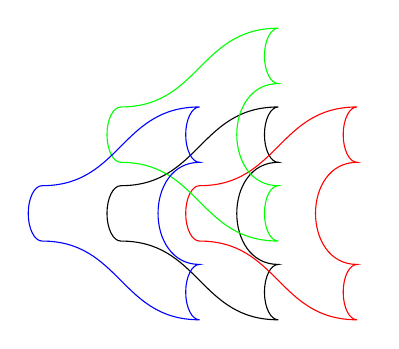
\begin{tikzpicture}[tqft/flow={east}]
\node[tqft/pair of pants,draw] at (0,0) {};
\node[tqft/pair of pants,draw,red] at (1,0) {};
\node[tqft/pair of pants,draw,green] at (0,1) {};
\node[tqft/pair of pants,draw,blue] at (-1,0) {};
\end{tikzpicture}

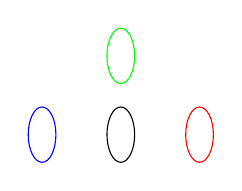
\begin{tikzpicture}[tqft/flow={east}]
\node[tqft boundary circle,draw] at (0,0) {};
\node[tqft boundary circle,draw,red] at (1,0) {};
\node[tqft boundary circle,draw,green] at (0,1) {};
\node[tqft boundary circle,draw,blue] at (-1,0) {};
\end{tikzpicture}

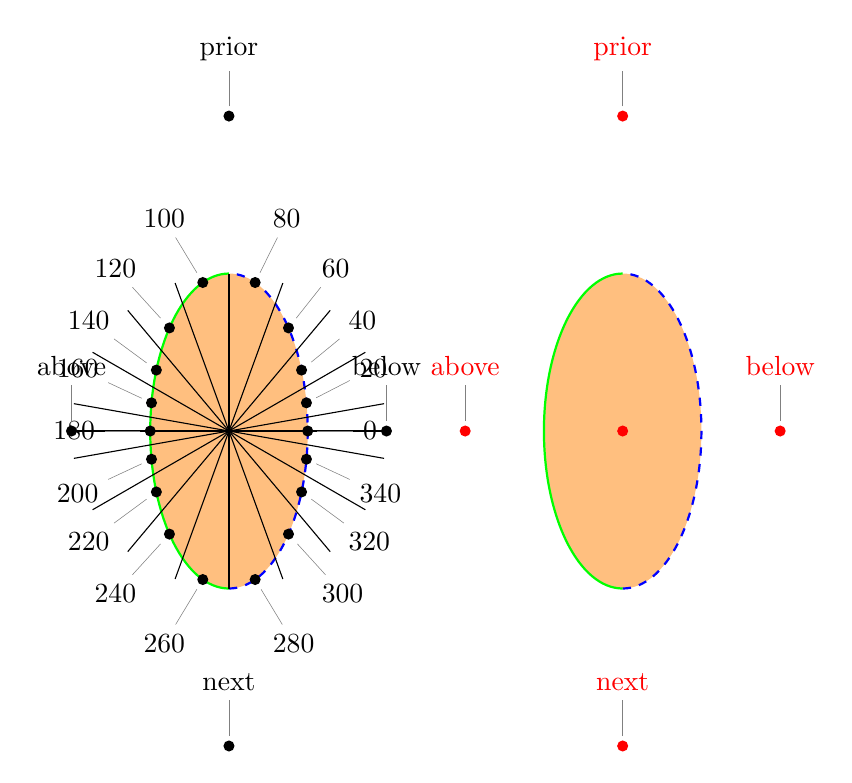
\begin{tikzpicture}[tqft/flow={east},every node/.style={tqft/cobordism style={draw,thick,red}}]
 \node[
   tqft boundary circle,
   tqft/circle width=2cm,
   tqft/circle depth=1cm,
   tqft/boundary separation=4cm,
   fill=orange,
   fill opacity=.5,
   tqft/boundary style={fill=purple},
   tqft/cobordism style={draw,thick,red},
   tqft/boundary lower style={draw,dashed,thick,blue},
   tqft/boundary upper style={draw,green,thick},
   tqft/incoming boundary components=4,
   tqft/outgoing boundary components=6,
   tqft/offset=-1.5,
 ] (a) {};
 \node[
   tqft boundary circle,
   tqft/circle width=2cm,
   tqft/circle depth=1cm,
   tqft/boundary separation=4cm,
   fill=orange,
   fill opacity=.5,
   tqft/boundary style={fill=purple},
   tqft/cobordism style={draw,thick,red},
   tqft/boundary lower style={draw,dashed,thick,blue},
   tqft/boundary upper style={draw,green,thick},
   tqft/incoming boundary components=4,
   tqft/outgoing boundary components=6,
   tqft/offset=-1.5,
 ] at (5,0) (b) {};
\fill[red] (b.centre) circle[radius=2pt];
 \fill[red] (b.next) circle[radius=2pt] node[pin=north:next] {};
 \fill[red] (b.prior) circle[radius=2pt] node[pin=north:prior] {};
 \fill[red] (b.above) circle[radius=2pt] node[pin=north:above] {};
 \fill[red] (b.below) circle[radius=2pt] node[pin=north:below] {};
 \fill (a.next) circle[radius=2pt] node[pin=north:next] {};
 \fill (a.prior) circle[radius=2pt] node[pin=north:prior] {};
 \fill (a.above) circle[radius=2pt] node[pin=north:above] {};
 \fill (a.below) circle[radius=2pt] node[pin=north:below] {};
 \draw (0,0) -- (90:2);
 \draw (0,0) -- (0:2);
 \draw (0,0) -- (180:2);
 \draw (0,0) -- (270:2);
\foreach \ang in {0,20,...,340} {
 \fill (a.\ang) circle[radius=2pt] node[pin=\ang:\ang] {};
 \draw (0,0) -- (270-\ang:2);
}
 \end{tikzpicture}

\end{document}